\chapter{PEC-L-Edge}
\label{chap_pec_l_edge}

\section{Introduction}

The iron opacity at conditions similar to the solar radiation/convection zone boundary was measured at the Sandia National Laboratory \citep{sandia_2015}, revealing wavelength-dependent opacity of 30--400\% higher than the predictions by theoretical opacity models.
To resolve this discrepancy, extensive close-coupling Breit--Pauli $R$-Matrix (BPRM) calculations have been carried out for \ion{Fe}{xvii} including 60 fine-structure levels within the $n\leq 3$ complexes in the \ion{Fe}{xviii} target ion \citep[60CC-BPRM,][]{60cc_2011} and 99 $LS$ terms within $n\leq 4$ (99LS-RM). They show strong photon absorption due to core excitation, resulting in an increment of 35\% in the Rosseland mean opacity over the Opacity Project (OP) data \citep [][hereafter NP16]{99cc_2016}. The convergence of photoionization cross section demonstrated in NP16 is criticized by \citet{more_comment_2017}, pointing out the underestimated photon absorption for levels with the outer electron of $n~>~4$. Such criticism is addressed in the current study. 

In section \ref{section_pec_l_edge}, the transition type that causes the jump of the background of the photoionization cross section in NP16 is identified. Such transitions occur around the same photon energy for each ion, and it turns out they are $99~Ry$, $106~Ry$ and $114~Ry$ for \ion{Fe}{xvii}, \ion{Fe}{xviii} and \ion{Fe}{xix}, respectively. The photoionization cross section due to these transitions is orders-of-magnitude larger than the other types of L-edge bound-free tansitions. To distinguish it from other types of L-edge transitions, we name it as PEC-L-Edge transition. In the same section, a systematic study is given for PEC-L-Edge transitions.


\section{PEC-L-Edge}
\label{section_pec_l_edge}
To identify the type of transitions that cause the jump of the background of photoionization cross section in BPRM calculation, we use FAC package \citep{gu_2008} to carry out the photoionization cross section including the same core configurations as those included in BPRM calculation, and match the bound levels by comparing the total angular momentum, parity, energy and photoionization cross section (see Section \ref{section_matching} for more details), and finally pick the transitions that contribute the most of photoionization cross section. In FAC, it outputs a table that lists all transitions, each of which is computed at six widespread points by default, and we consider the photoionization cross section at the first default point in the order of $0.01~Mb$ as large. In the rest of this section I will give a few examples of PEC-L-Edge transitions, followed by a systematic study of their ionization thresholds and photoionization cross section for \ion{Fe}{xvii}, \ion{Fe}{xviii} and \ion{Fe}{xix}.

\subsection{PEC-L-Edge in BPRM and RDW}
To give a clear illustration of PEC-L-Edge transitions, we take the ground state of \ion{Fe}{xvii} as an example (see figure \ref{fig_fe17_ground}). In the current BPRM (see Chapter \ref{chap_bprm_fe17_fe18}) calculation for \ion{Fe}{xvii}, the core configurations included are ${2s^2 2p^5}$, ${2s 2p^6}$, ${2s^2 2p^4 n\ell}$, ${2s 2p^5 n\ell}$, ${2p^6 3\ell'}$, where $n=3, ~4$, and $\ell,~ \ell'\leq2$, which result in 218 fine structure levels of the core. In the RDW calculation, the same core configurations are included. After extracting the transitions that give the large photoionization cross section, we find the final ionized states are the three levels in ${2s^2 2p^5}$ and ${2s 2p^6}$, and their ionization thresholds are $92.3~Ry$, $93.2~Ry$ and $102.3~Ry$. Though there are no electrons outside of L-shell, we can still treat one $2p$ electron as the outer electron, and the rest $2s,~2p$ electrons belong to the core. Thus PEC-L-Edge transitions happen when only one $2s$ or $2p$ electron is ionized, keeping the other electrons unchanged. In figure \ref{fig_fe17_ground}, the three PEC-L-Edge transitions successfully reproduce the background of BPRM calculation. Though there are many transitions above $150~Ry$, they are negligibly small when compared with the PEC-L-Edge transitions.

%======Figure Fe17_ground
\begin{figure}
	\centering
	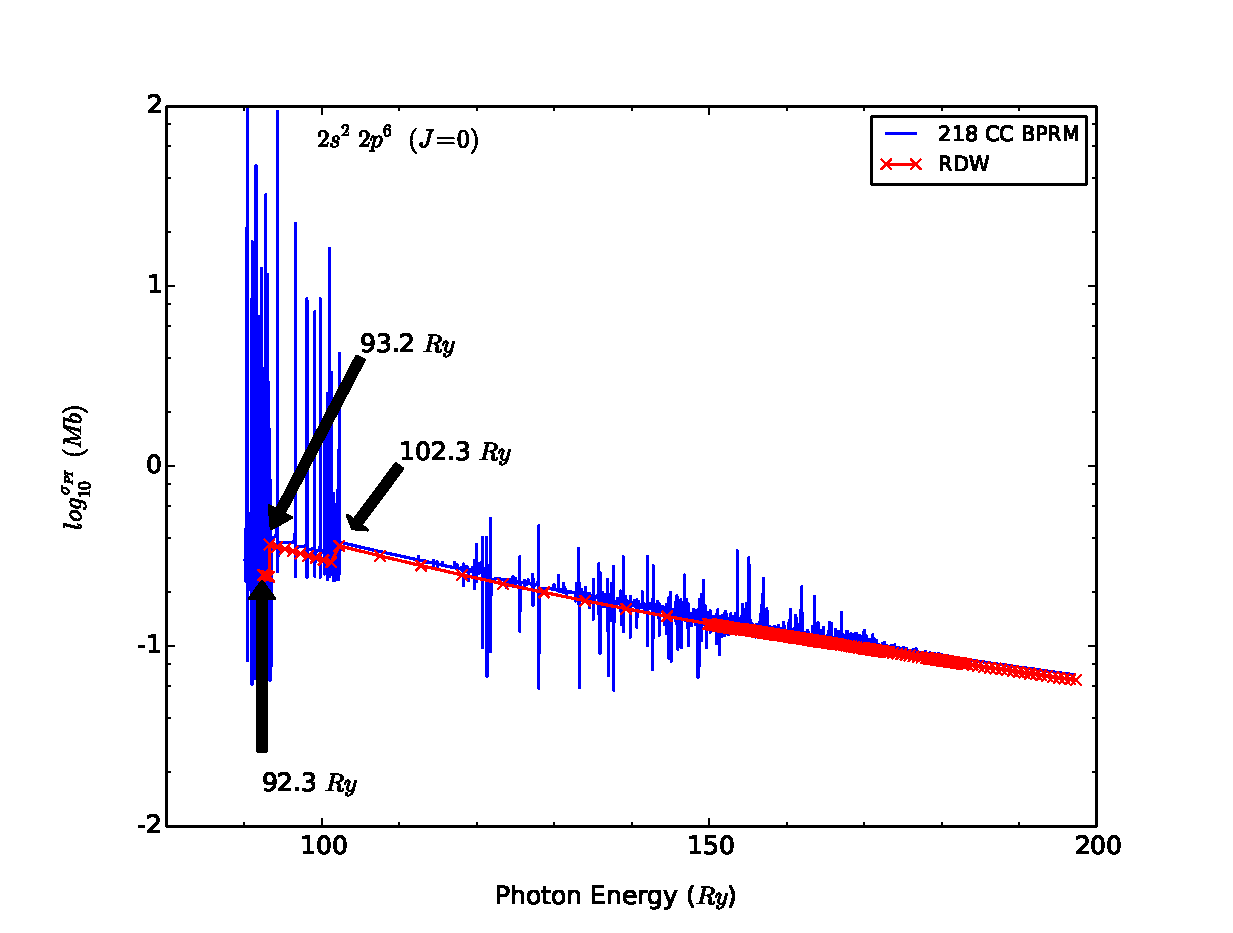
\includegraphics[width=\textwidth]{figures_5/fe17_ground.eps}	
	\caption{The photoionization of the ground state of \ion{Fe}{xvii}. The three PEC-L-Edge transitions using FAC reproduce the background of the photoionization cross section in BPRM calculation. The thresholds of these PEC-L-Edge transitions are marked. The energy mesh is created such that 10 points are uniformly distributed between adjacent thresholds.}
	\label{fig_fe17_ground}
\end{figure}

In the current \ion{Fe}{xviii} BPRM calculation (see Chapter \ref{chap_bprm_fe17_fe18}), the core configurations included are $2s^2 2p^4$, $2s 2p^5$, $2p^6$, $2s^2 2p^3 3\ell$, $2s 2p^4 3\ell$, $2s^2 2p^3 4\ell$, where $\ell\leq2$, which yield 276 fine structure levels of the core. Since the core configurations of $n=3$ and $n=4$ are not completely included, some bound levlels with the outer electron in M- or N-shell will not get the full contribution from PEC-L-Edge transitions. For example, for level $2s^22p^44d~(J=5/2)$ in figure \ref{fig_fe18_5_0_20}, the top panel shows excellent reproduction of the background by RDW, showing various steps before coming to a big jump, though the energies are off a tiny bit. By extracting the main transitions in FAC, we find the jump is due to the PEC-L-Edge transitions to levels in $2s^2 2p^3 4d$. When doing the top up calculation for this level (see Section \ref{section_other_targets}), we extend the BPRM data to higher energy region using RDW data (the dash-dotted line in the bottom panel), which is mainly due to the PEC-L-Edge transitions to levels in $2s^2 2p^3 4d$, and add the contribution from other unincluded core configurations up to $n=10$ (the black line in the bottom panel), which is mainly due to the PEC-L-Edge transitions to levels in $2s 2p^4 4d$. 

In the current \ion{Fe}{vii} and \ion{Fe}{xviii} BPRM calculation, all such jumps are reproduced by RDW calculation (see \url{https://github.com/zhao1157/PhD-Atomic-Physics/tree/master/fe17\_fe18\_matched\_levels}), and we believe the type of transitions that cause such jump of background is identified, i.e. PEC-L-Edge transition, which falls in the spectator-electron process category \citep{mendoza_2018}. In \citet{mendoza_2018}, the study case on the K-edge of \ion{O}{vi} can be explained in the similar way like PEC-L-Edge in our study. As for the high-n levels that do not show such PEC-L-Edges, the top up calculation complements such missing jumps (see figure \ref{fig_fe17_fe18_other_jump}). In both  \ion{Fe}{vii} and \ion{Fe}{xviii} BPRM calculations, the core configurations included do not have $n>4$, so the bound levels with outer electron of $n=5,~7$ do not have PEC-L-Edges in BPRM calculation. In the top up calculation, we consider all bound levels with $n\leq10$, so we include the core configurations with $n\leq10$ in order to obtain the PEC-L-Edge for each level.

In NP16, the convergence of the photoionization cross section is demonstrated by showing two levels which have such PEC-L-Edge background that dominates most of the resonances in the higher energy region, however, there are many other levels that do not have such PEC-L-Edge background, for example figure 4(b) in NP16, which is correctly pointed out by \citet{more_comment_2017} that it is due to missing $n>4$ core configurations, thus it is not sufficient to prove the convergence of the photoionization cross section by considering only two levels. And the enhancement obtained by 99LS-RM over 60CC-BPRM (or 30CC as referred to in NP16) calculation for the two levels shown in figure 3(b, c) in NP16 is due to the core configurations $2s2p^53p$ and $2s2p^53d$, which are not included in 60CC-BPRM, but in 99LS-RM. In the current BPRM calculation complemented by RDW calculation, all bound levels have such PEC-L-Edge backgound starting around $100~Ry$, thus the photoionization cross section is converged. In the rest of this section, I will show two properties that are very important to PEC-L-Edge transitions.

%======Figure fe18_5_0_20
\begin{figure}
	\centering
	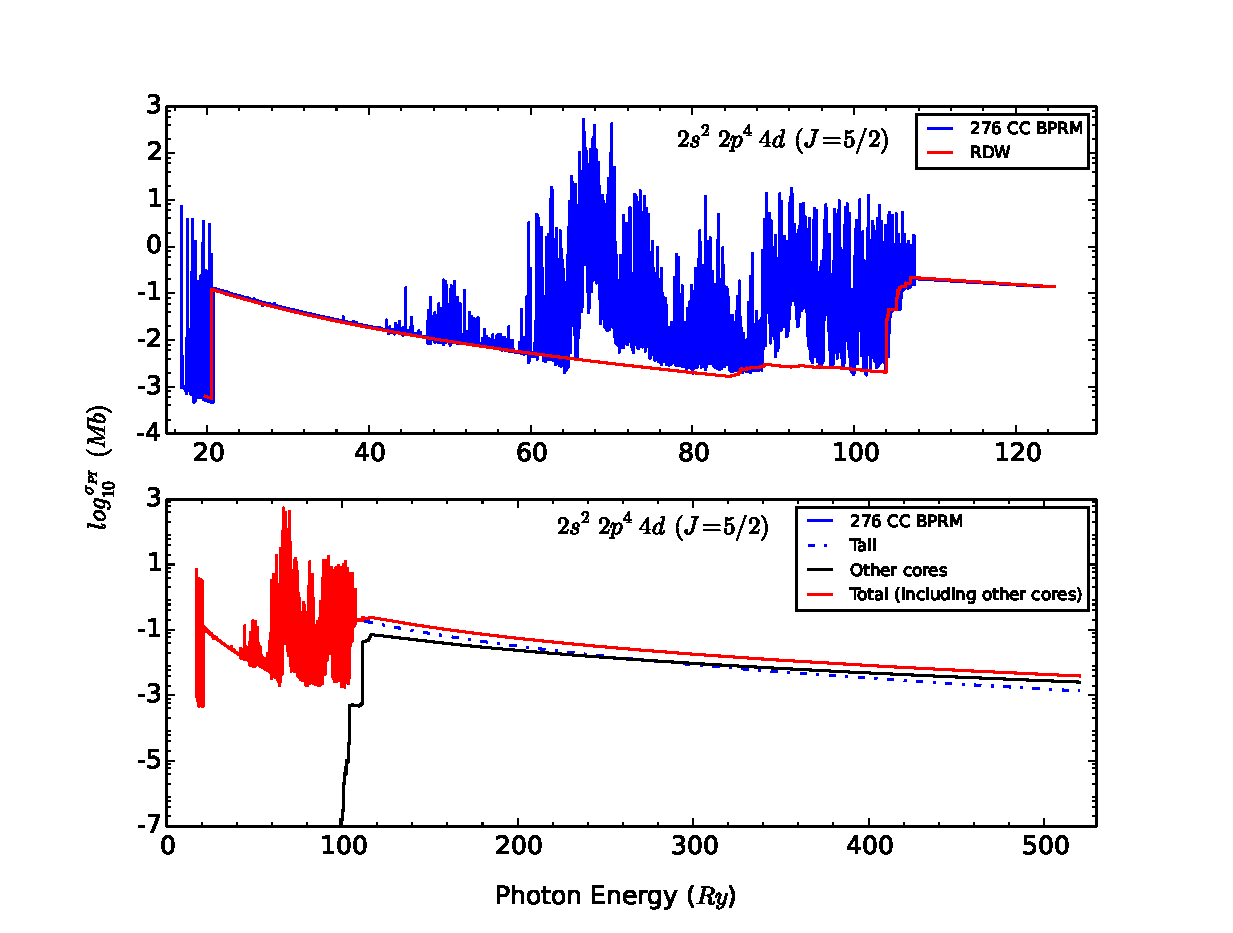
\includegraphics[width=\textwidth]{figures_5/fe18_5_0_20}	
	\caption{The photoionization cross section of level $2s^22p^44d~(J=5/2)$ in \ion{Fe}{xviii}. In the top panel, RDW calculation reproduces the background of BPRM calculation; in the bottom panel, the BPRM calculation is extended with a tail in higher energy region (blue dash-dotted line) using RDW and the contribution from other core configurations up to $n=10$ (black line) is added, giving the total photoionization cross section (red line).}
	\label{fig_fe18_5_0_20}
\end{figure}

%======Figure fe17_fe18_other_jump
\begin{figure}
	\centering
	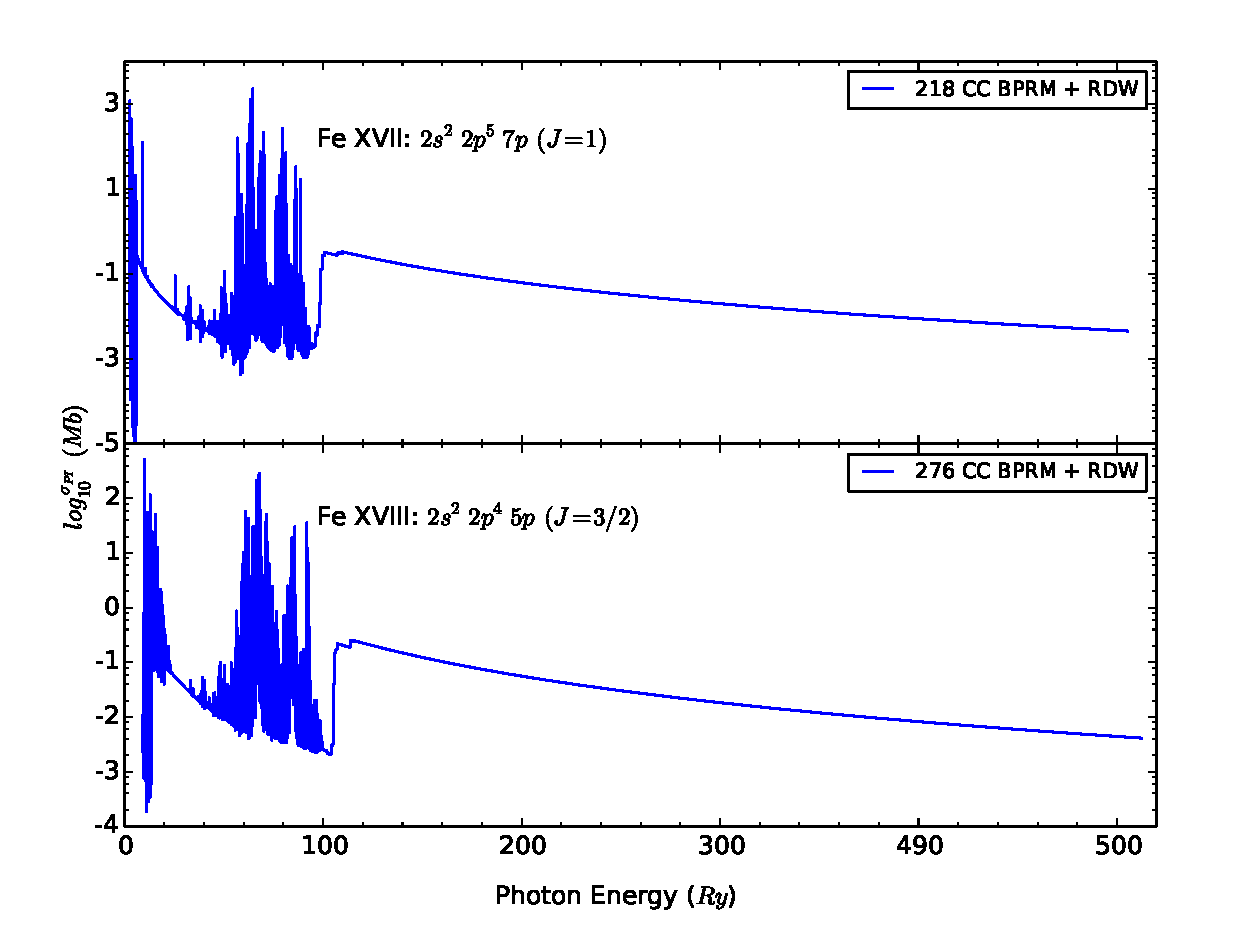
\includegraphics[width=\textwidth]{figures_5/fe17_fe18_other_jumps}	
	\caption{The photoionization cross section of level $2s^22p^57p~(J=1)$ in \ion{Fe}{xvii} and level $2s^22p^45p~(J=3/2)$ in \ion{Fe}{xviii}. The PEC-L-Edge shows up in both levels when high-n core configurations are included in the top up calculation.}
	\label{fig_fe17_fe18_other_jump}
\end{figure}

\subsection{Properties of PEC-L-Edge}
\label{section_propertie_pec_l_edge}
Pure RDW calculations are carried out for \ion{Fe}{xvii}, \ion{Fe}{xviii} and \ion{Fe}{xix} to study the properties of these PEC-L-Edge transitions, and we find for each ion, the PEC-L-Edge background starts around the same photon energy, i.e. $100~Ry$, $106~Ry$ and $114~Ry$ for  \ion{Fe}{xvii},  \ion{Fe}{xviii} and \ion{Fe}{xix}, respectively. And the photoionization cross section is large and varies little from level to level.

To demonstrate the PEC-L-Edge transitions occurring around the same photon energy, see diagram \ref{fig_fe17_fe18_fe19_thresholds}. Since the PEC-L-Edge transitions only ionize one electron from $2s$ or $2p$ subshell, while keeping ther other electrons as spectators, the ionization threshold is 
\begin{align}
\label{equ_ionization}
\Delta E (Ry)&= \Delta I - \frac{(z+1)^2}{n^2} + \frac{z^2}{n^2} \nonumber  \\
 			   &= \Delta I - \frac{1+2z}{n^2}.
\end{align}
For \ion{Fe}{xvii}, \ion{Fe}{xviii} and \ion{Fe}{xix}, $z = 17,~18,~19$, respectievly, and $n$ takes intergers from 2 to 10, thus the second term in equation \ref{equ_ionization} is approximately less than $1~Ry$ when $n\geq6$ and this proves the ionization thresholds being around the same value for each ion. When $n=2$, the second term gives a difference of $8.75~Ry$, $9.25~Ry$ and $9.75~Ry$ for  \ion{Fe}{xvii}, \ion{Fe}{xviii} and \ion{Fe}{xix}, respectively.

%======Figure ionization_threshold
\begin{figure}
	\centering
	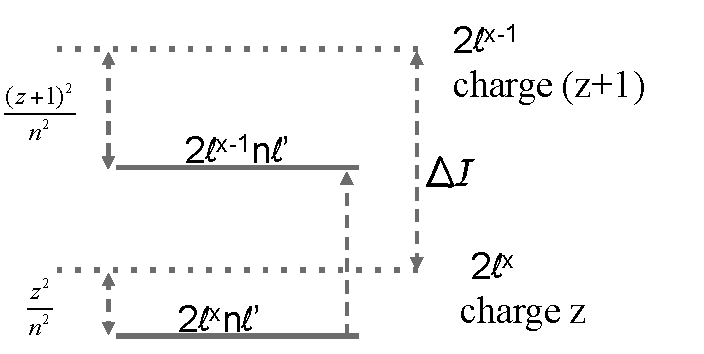
\includegraphics[width=.9\textwidth]{figures_5/ionization_energy}	
	\caption{The diagram of ionization threshold of PEC-L-Edge transitions. PEC-L-Edge transitions only happen between initial level in configuration $2\ell^x~n\ell'$ and final level in $2\ell^{x-1}~n\ell'$, and the ionization threshold is denoted by $\Delta E$. $\Delta I$ is the energy difference between core configurations $2l^x$ and $2l^{x-1}$, and the energy of level $2\ell^x~n\ell'$ is $\frac{z^2}{n^2}$ below the core  $2l^x$, and the energy of level $2\ell^{x-1}~n\ell'$ is $\frac{(z+1)^2}{n^2}$ below the core  $2l^{x-1}$.}
	\label{fig_fe17_fe18_fe19_thresholds}
\end{figure}

%======Figure ionization_threshold_start_end
\begin{figure}
	\centering
	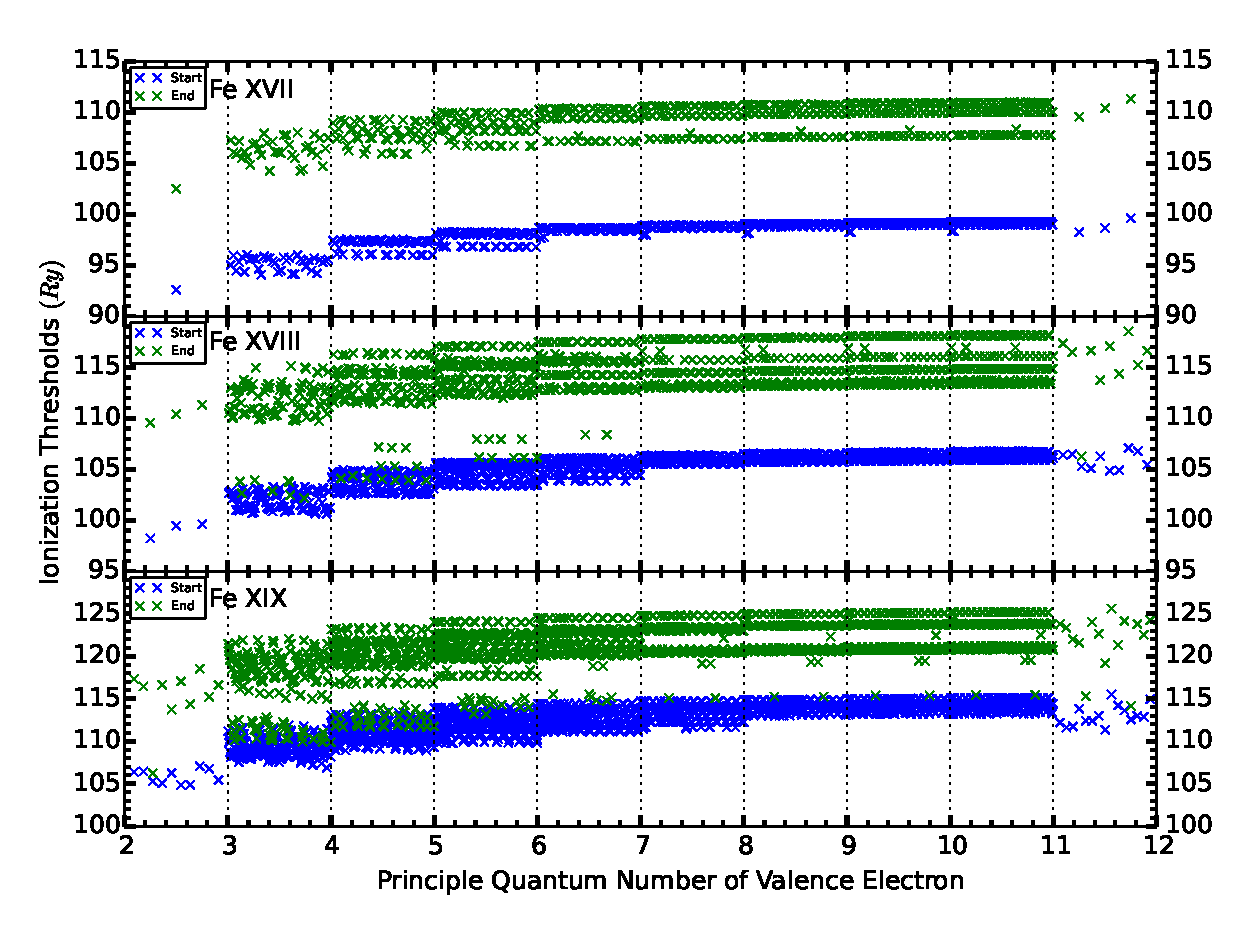
\includegraphics[width=\textwidth]{figures_5/fe17_fe18_start_end}	
	\caption{The thresholds of PEC-L-Edge transitions for  \ion{Fe}{xvii}, \ion{Fe}{xviii} and \ion{Fe}{xix} in pure RDW calculation. Blue ``$\times$'' refers to the lowest (starting) threshold of PEC-L-Edge transition and green ``$\times$'' the highest (ending) threshold of PEC-L-Edge transition. In region 11-12, these data points are for the core configurations without the outer electron.}
	\label{fig_fe17_fe18_fe19_thresholds_start_end}
\end{figure}

%======Figure fe17_fe18_fe19_end_500_PI
\begin{figure}
	\centering
	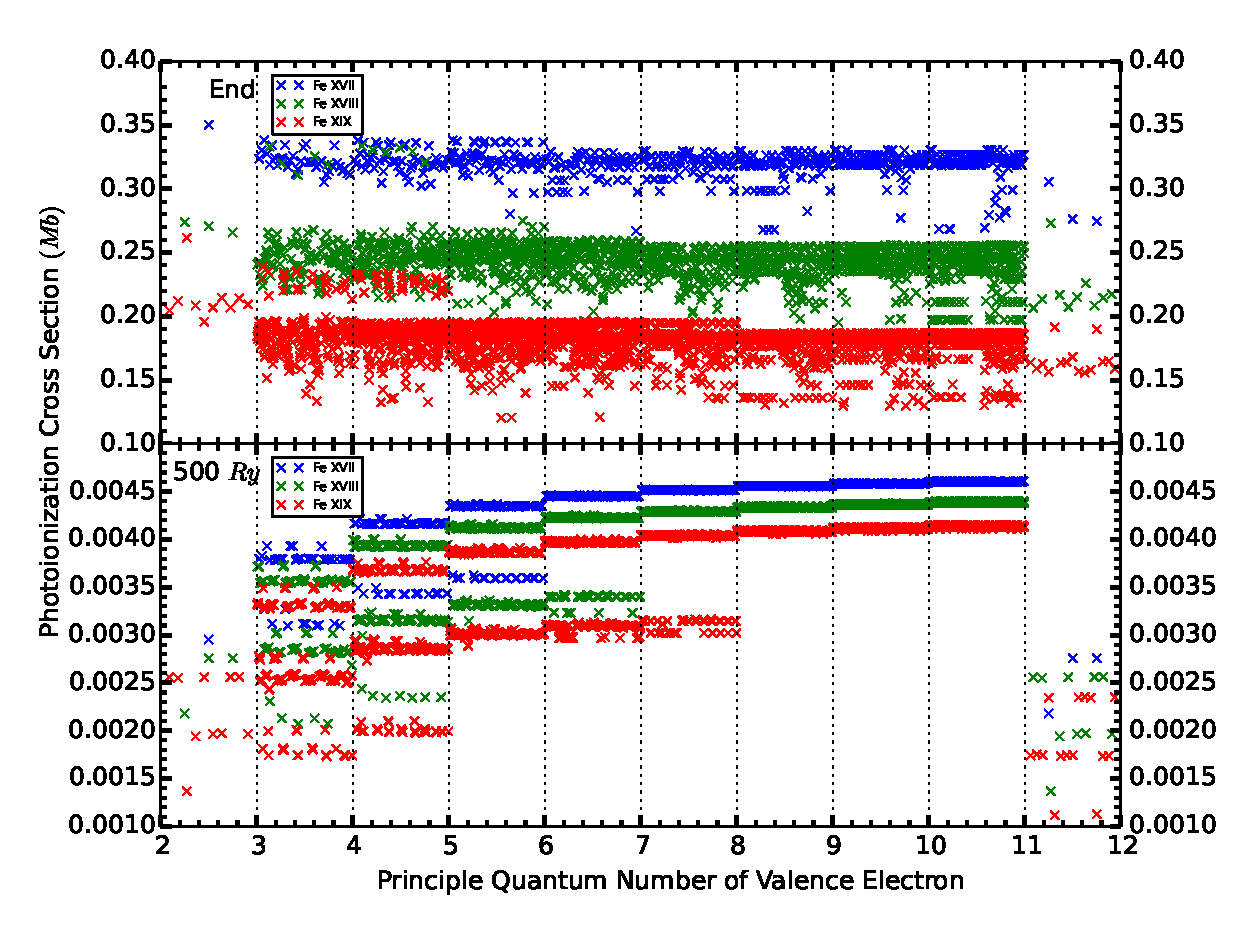
\includegraphics[width=\textwidth]{figures_5/fe17_fe18_end_500}	
	\caption{The photoionization cross section of PEC-L-Edge transitions for  \ion{Fe}{xvii}, \ion{Fe}{xviii} and \ion{Fe}{xix} at energies just above the thresholds denoted by``End'' in figure \ref{fig_fe17_fe18_fe19_thresholds_start_end} and at $500~Ry$. In region 11-12, these data points are for the core configurations without the outer electron and the photoionization cross section in the top panel is the maximum value above the lowest PEC-L-Edge threshold.}
	\label{fig_fe17_fe18_fe19_pi_end_500ry}
\end{figure}

In the pure RDW calculation, we consider all bound levels with the principle quantum number of the outer electron within 10, so in order to get PEC-L-Edge background for each level, the core configurations with $n\leq10$ are included and only same-n-complex configuration interaction for bound and core configurations is considered. The number of bound levels for  \ion{Fe}{xvii}, \ion{Fe}{xviii} and \ion{Fe}{xix} is 587, 1590 and 2613, respectively. In figure \ref{fig_fe17_fe18_fe19_thresholds_start_end}, the lowest threshold (blue ``$\times$'') of PEC-L-Edge transition is plotted against the principle quantum number of the outer electron. For all levels with the same quantum number $n$ of the outer electron, they are uniformly distributed in region ($n,~n+1$). In region (11, 12), these points are for the core configurations with the outer electron removed. Just as equation \ref{equ_ionization} predicts, the PEC-L-Edge transitions start around the same energy for $m\geq6$, and $\Delta I$ is $99~Ry$, $106~Ry$ and $114~Ry$ for \ion{Fe}{xvii}, \ion{Fe}{xviii} and \ion{Fe}{xix}, respectively, which approaches the ionization thresholds of the core without the outer electron, as shown in region (11, 12). For low-n bound levels, for example $n=2$, the lowest ionization threshold is $93~Ry$, $98~Ry$ and $105~Ry$ for \ion{Fe}{xvii}, \ion{Fe}{xviii} and \ion{Fe}{xix}, respectively, which falls around the region predicted by equation \ref{equ_ionization}. To study the photoionization cross section due to PEC-L-Edge transitions in higher-energy region, we calculate it at energy just above the highest threshold of PEC-L-Edge transition for each level (denoted by green ``$\times$'' in figure \ref{fig_fe17_fe18_fe19_thresholds_start_end}) and at $500~Ry$ and the result is shown in figure \ref{fig_fe17_fe18_fe19_pi_end_500ry}. For each ion, the photoionization cross section fluctuates in a small region at energies marked as ``End'' and at $500~Ry$, and values in between approximately follow  as \(\sigma(\nu) \propto E^{-3}\). It is almost independent of the outer electron, and it is a little higher than the result of the core configurations with the outer electron removed.




\section{Conclusion}
The type of strong dipole-allowed transitions in L-shell photoionization cross section in BPRM calculation is identified by RDW calculation, i.e. PEC-L-Edge transition type, which ensures the large PEC-L-Edge background for all bound levels that are considered in the current BPRM+RDW calculation (see Chapter \ref{chap_topup}). Two properties of the PEC-L-Edge transitions for \ion{Fe}{xvii}, \ion{Fe}{xviii} and \ion{Fe}{xix} are investigated, one of which is roughly the same starting threshold of PEC-L-Edge transition for high-n levels, i.e. $99~Ry$ for \ion{Fe}{xvii}, $106~Ry$ for \ion{Fe}{xviii} and $114~Ry$ for \ion{Fe}{xix}, and the other is that the PEC-L-Edge background dominates in the high-energy region and is not much affected by the high-n outer electron.


